\chapter[Verification and Validation]{Verification and Validation}
\label{ch:ch4results}

%% The following annotation is customary for chapter which have already been
%% published as a paper.
\blfootnote{}

\begin{abstract}
%abstract
In this chapter, the different features of the new pressure based solver will be verified and validated against analytical solutions, experimental data and other references. For verification of the solver, problems with an analytical solution like the Taylor-Couette flow and the plane Poisuelle flow will be used. The validation cases presented will be used to test the different features that are typically encountered during external aerodynamics applications. First, laminar flow problems are used to validate the implementation of the flow solver. Then, turbulent flow problems are presented to validate the coupling of the new flow solver with the existing turbulence solvers. Finally, the unsteady behavior of the new solver is validated. Wherever possible the grids for the numerical simulations are taken from standard sources like the NASA turbulence modeling database~\cite{NASATMR} or the SU2 test case repository to avoid any potential sources of error from mesh generation.

Laminar and turbulent boundary layers are extremely crucial in wind turbine aerodynamics and the numerical solutions from the new solver are validated against theoretical boundary layer solutions under both circumstances. Flow separation, though undesirable, occurs frequently and the behavior of the new solver under separated conditions is tested for the flow over a backward facing step for both laminar and turbulent flow conditions. Other representative test cases, like the flow over a cylinder and flow past an airfoil are also presented. Finally, two unsteady cases are considered; a laminar flow past a square cylinder and a turbulent flow past a pitching airfoil undergoing dynamic stall. 
\end{abstract}
\section{Verification} 
In order to verify the accuracy of the solver, Couette flow or the flow between two solid surfaces is simulated. Two special cases are considered here - the flow between two concentric infinitely long rotating cylinders (also known as Taylor-Couette flow, see the figure~\ref{fig:couetteschem}) and a planar flow between two solid infinitely long parallel plates that are held fixed (also known as plane Poisuelle flow, see figure~\ref{fig:channelschem}). An analytical solution for the velocity profile can be found for both these cases which is used to calculate the order of convergence of the solver. 

While an analytical solution is not available for the laminar flow in a lid driven cavity, reference solutions for velocity can be found in literature~\cite{Ghia1982}. Thus, the solutions for the lid driven cavity is also used to compute the order of accuracy.

\subsubsection{Taylor Couette flow}
The schematic of the Taylor-Couette flow is shown in figure~\ref{fig:couetteschem}. 
\begin{figure}[h]
    \centering
    \captionsetup{justification=centering}
    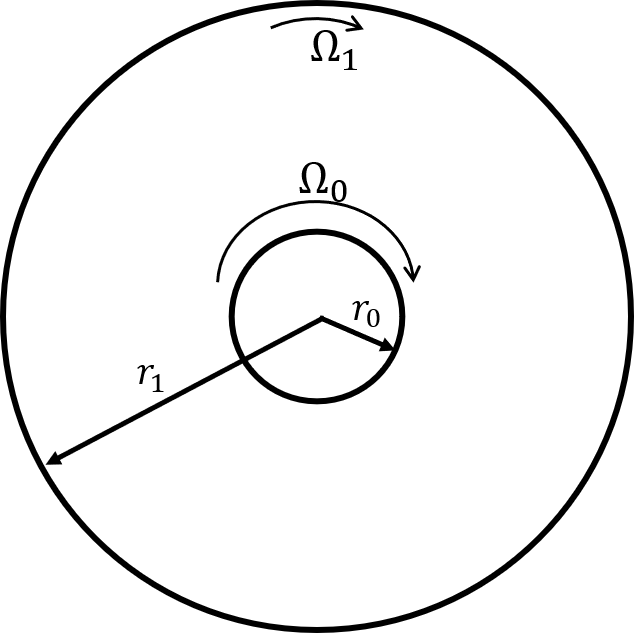
\includegraphics[width=0.25\textwidth]{figures/couette_schem.png}
    \caption{Schematic of the Taylor-Couette flow.}
     \label{fig:couetteschem}
\end{figure}
The inner cylinder has a radius of $r_0$ and the outer radius is $r_1$. $\Omega_0$ and $\Omega_1$ are the angular velocities of the inner and outer cylinders respectively. The analytical solution~\cite{taylor1923viii} for the azimuthal velocity as a function of the radius $r$ is
\begin{equation}
    u_{ana}(r) = r_0 \Omega_0 \frac{r_1/r - r/r_1}{r_1/r_0-r_0/r_1} + r_1 \Omega_1 \frac{r/r_0 - r_0/r}{r_1/r_0-r_0/r_1}.
\end{equation}{}
\begin{figure}[h]
    \centering
     \captionsetup{justification=centering}
    \begin{subfigure}[b]{0.47\textwidth}
    \captionsetup{justification=centering}
        \includegraphics[width=1.0\textwidth]{figures/Velocity_Couette.eps}
        \caption{Velocity vs radial distance.}
        \label{fig:couettevel}
    \end{subfigure}
    ~ %add desired spacing between images, e. g. ~, \quad, \qquad, \hfill etc. 
      %(or a blank line to force the subfigure onto a new line)
    \begin{subfigure}[b]{0.47\textwidth}
    \centering
    \captionsetup{justification=centering}
        \includegraphics[width=1.0\textwidth]{figures/Error_Couette.eps}
        \caption{Order of convergence.}
        \label{fig:couetteerr}
    \end{subfigure}
    \caption{Grid convergence for the Taylor Couette flow.}
\end{figure}

The simulation was carried out on a domain with $r_0 = 1m$ and $r_1=5m$. The outer wall is held fixed ($\Omega_1 = 0$) and the inner wall is rotating at an angular velocity $\Omega_0 = 1$ rad$/$s. The two solid walls are treated as moving wall boundaries. Three different grid resolutions are considered with $16$, $32$ and $64$ cells along the radial direction and with $40$ nodes along the circumference of the cylinders. Uniform grid spacing is used in all cases. 

Figure~\ref{fig:couettevel} shows the comparison between the numerical and analytical velocity profile. The numerical solution matches the analytical solution for all the grid resolutions very well. The numerical error is computed as 
\begin{equation*}
e_{num} = |u_{ana} - u_{num}|.
\end{equation*} 
Figure~\ref{fig:couetteerr} shows the $log_{10}$ of the $L_2$ norm of the error plotted against the number of points in the radial direction.  The numerical error decreases at a rate of $1.938$ indicating an approximately second order rate of convergence as the grid size is halved.

\paragraph{Convergence behavior}
The residual history for the grids with $32$ and $64$ nodes are plotted in figures~\ref{fig:couetteres32} and \ref{fig:couetteres64}. The residuals of both the velocity components and the mass flux, which serves as the indicator for convergence of the continuity equation, all converge within $1200$ iterations for the coarser grid and about $4400$ iterations for the fine grid.
\begin{figure}[h]
    \centering
     \captionsetup{justification=centering}
    \begin{subfigure}[b]{0.48\textwidth}
    \captionsetup{justification=centering}
        \includegraphics[width=1.0\textwidth]{figures/couette_conv_32.eps}
        \caption{$40\times32$ grid.}
        \label{fig:couetteres32}
    \end{subfigure}
    ~ %add desired spacing between images, e. g. ~, \quad, \qquad, \hfill etc. 
      %(or a blank line to force the subfigure onto a new line)
    \begin{subfigure}[b]{0.48\textwidth}
    \centering
    \captionsetup{justification=centering}
        \includegraphics[width=1.0\textwidth]{figures/couette_conv_64.eps}
        \caption{$40\times64$.}
        \label{fig:couetteres64}
    \end{subfigure}
    \caption{Convergence history for the Taylor Couette flow residual.}
\end{figure}
The two velocity components converge identically because of rotational symmetry.

\subsubsection{Plane Poisuelle flow}
The plane Poisuelle flow is the flow between two infinitely long parallel plates that are held fixed (figure~\ref{fig:channelschem}). The boundary conditions used for the simulation are shown in figure~\ref{fig:channelbcs}. At the inlet boundary, a uniform velocity profile is prescribed, and a zero velocity gradient at the outlet is specified. The outlet pressure is set to zero. A small symmetry region is present immediately after the inlet before the channel starts.
\begin{figure}[h!]
    \centering
    \captionsetup{justification=centering}
    \begin{subfigure}[b]{0.47\textwidth}
    \centering
    \captionsetup{justification=centering}
    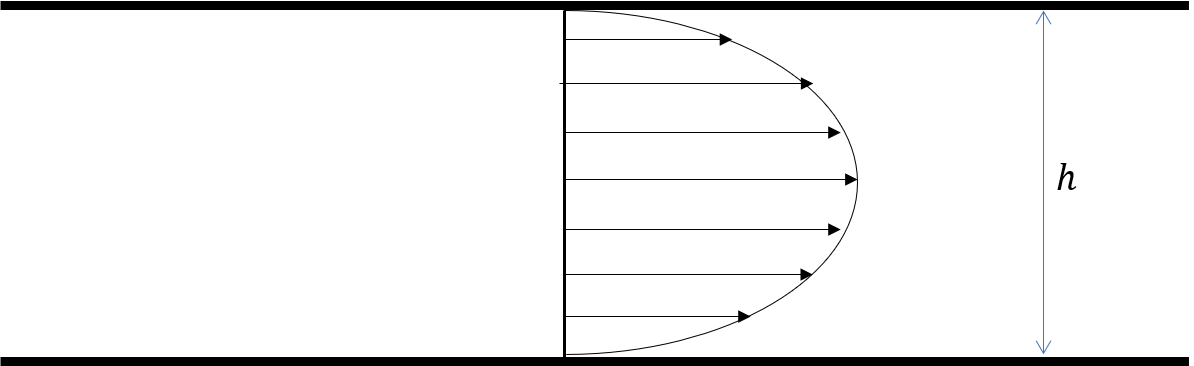
\includegraphics[width=1.0\textwidth]{figures/channel_schem.png}
    \caption{Schematic of the plane Poisuelle flow.}
     \label{fig:channelschem}
    \end{subfigure}
    ~ %add desired spacing between images, e. g. ~, \quad, \qquad, \hfill etc. 
      %(or a blank line to force the subfigure onto a new line)
    \begin{subfigure}[b]{0.47\textwidth}
    \centering
    \captionsetup{justification=centering}
     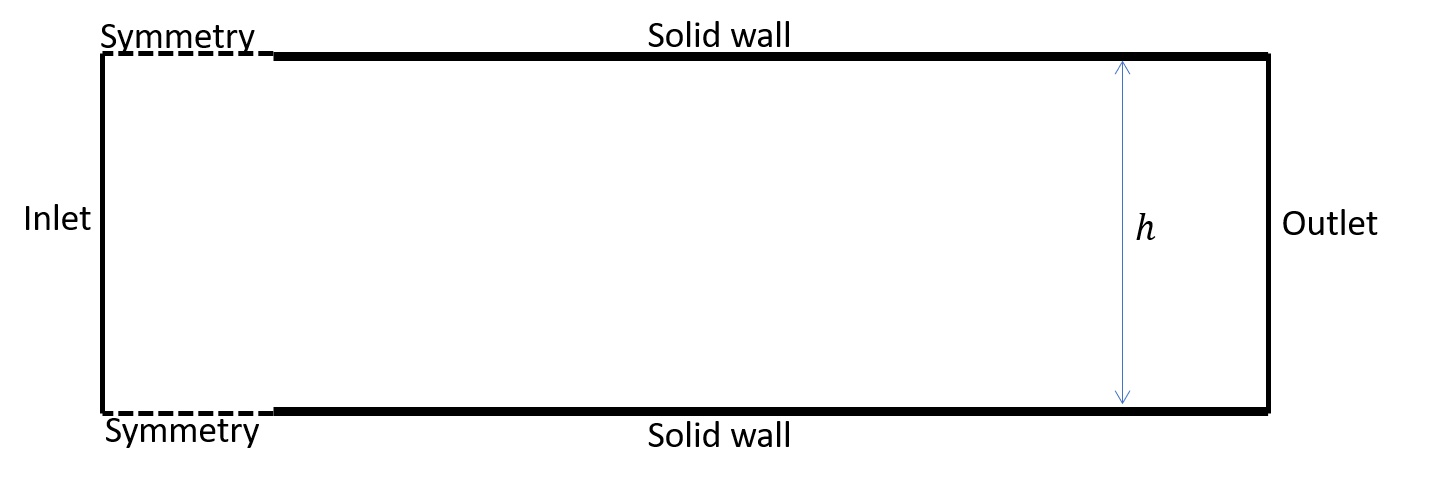
\includegraphics[width=1.0\textwidth]{figures/channel_bcs.png}
    \caption{Domain and boundary conditions.}
     \label{fig:channelbcs}
    \end{subfigure}
    \caption{(a) Schematic of the plane Poisuelle flow and (b) the domain and boundary conditions for the numerical simulation.}
\end{figure}
The plane Poisuelle flow at a mean flow Reynolds number based on channel width $h$ and inlet velocity $U_{in}$ of $Re = \frac{h U_{in}}{\nu} = 400$ is considered. For fully developed flow conditions, the axial velocity profile at any location $y$ can be computed as
\begin{equation}
    u(y)=-\frac{dP}{dx}\frac{1}{2\mu}y(y-h),\qquad 0\leq y \leq h
\end{equation}{}

\noindent where $\frac{dP}{dx}$ is the constant pressure gradient in the streamwise direction, $\mu$ is the laminar viscosity and $h$ is the channel width.
The domain is $1.25 m$ long in the streamwise direction with a symmetry region of $0.25 m$ after the inlet boundary. The distance between the two solid walls is $h=0.125 m$ (figure~\ref{fig:channelbcs}). Four different mesh resolutions are chosen with $16$, $32$, $64$ and $128$ elements in the direction normal to the solid walls and $100$ elements in the streamwise direction. 

\begin{figure}[h!]
    \centering
    \captionsetup{justification=centering}
    \begin{subfigure}[b]{0.45\textwidth}
    \centering
    \captionsetup{justification=centering}
        \includegraphics[width=1.0\textwidth]{figures/channel_vel.eps}
        \caption{Velocity comparison.}
        \label{fig:chvelcmp}
    \end{subfigure}
    ~ %add desired spacing between images, e. g. ~, \quad, \qquad, \hfill etc. 
      %(or a blank line to force the subfigure onto a new line)
    \begin{subfigure}[b]{0.45\textwidth}
    \centering
    \captionsetup{justification=centering}
        \includegraphics[width=1.0\textwidth]{figures/channel_l2.eps}
        \caption{$L_2$ norm of the error}
        \label{fig:chl2}
    \end{subfigure}
    \caption{(a) Comparison of numerical and analytical results. (b) Error as a function of number of cells.}
\end{figure}
Figure~\ref{fig:chvelcmp} shows the comparison of the streamwise velocity at $x=0.9$, which is $7.2h$ away from the start of the channel, as a function of the normal distance for different grid resolutions against the analytical solution. The flow is fully developed after roughly $5h$ to $6h$ from the start of the channel. The pressure gradient required to compute the numerical solution is obtained from the results of the finest grid with $128$ elements in the normal direction. The numerical results from all the grids match the analytical solution closely. The error between the numerical solution and the analytical solution is computed for the three meshes with $16$, $32$ and $64$ elements. The $L_2$ norm of the error is plotted against the number of elements in the normal elements in the figure~\ref{fig:chl2} on a log scale. The slope of the error curve is $2.1$.

\paragraph{Convergence behavior}
\begin{figure}[h]
    \centering
    \captionsetup{justification=centering}
    \begin{subfigure}[b]{0.47\textwidth}
    \captionsetup{justification=centering}
        \includegraphics[width=1.0\textwidth]{figures/channel_conv_hist.eps}
        \caption{SIMPLE convergence history.}
        \label{fig:channelhist}
    \end{subfigure}
    ~ %add desired spacing between images, e. g. ~, \quad, \qquad, \hfill etc. 
      %(or a blank line to force the subfigure onto a new line)
    \begin{subfigure}[b]{0.47\textwidth}
    \centering
    \captionsetup{justification=centering}
        \includegraphics[width=1.0\textwidth]{figures/channel_conv_comparison.eps}
        \caption{SIMPLEC and SIMPLE.}
        \label{fig:channelcmp}
    \end{subfigure}
    \caption{Plane Poisuelle flow  (a) residual convergence history on the $100\times64$ grid and (b) comparsion of convergence behavior for SIMPLE and SIMPLEC for the streamwise velocity on the $100\times64$ grid.}
\end{figure}
Figure~\ref{fig:channelhist} shows the convergence history for the two velocity components and the mass flux for the SIMPLE algorithm. Convergence is achieved in $630$ iterations. Figure~\ref{fig:channelcmp} shows the comparison of residual convergence of the streamwise velocity component for the SIMPLE and SIMPLEC iterative methods. Since the pressure corrections are under-relaxed appropriately, there is no significant difference in convergence behavior. However, SIMPLEC does converge slightly faster in this case.

\subsubsection{Lid driven cavity}
The flow within a lid driven cavity is a commonly used validation problem for CFD solvers. The domain consists of a square cavity with the top wall being moved at a constant velocity along the $x$ axis. This case also serves to test the moving wall boundary condition. While there is no analytical solution for this case, the results from a lid driven cavity are compared against results from Ghia~\cite{Ghia1982}. Ghia~\cite{Ghia1982} solves the vorticity stream function formulation of the incompressible Navier Stokes equations using a multigrid method. The flow is steady and laminar and is a solution of the exact Navier Stokes equation. A square domain $L\times L$ with side $L=1m$ is used. The top wall of the domain is moving at a constant velocity, $U_w$, in the $x$ direction. The flow Reynolds number defined based on the wall velocity, $U_w$ and the length of side of the square lid is $Re= \frac{U_w L}{\nu} = 400$. Three different grids are considered with $33$, $65$ and $129$ nodes along each direction. A uniform grid spacing is used throughout the domain. 
Figure~\ref{fig:ldcgr} shows the $x$ component of the velocity along $x=0.5$ for the three grids and the benchmark results from Ghia~\cite{Ghia1982}. The numerical results improve against the benchmark solution as the grid is refined. Figure~\ref{fig:ldcstr} shows the $L_2$ norm of the error between the results from SU2 and the benchmark solution. The error reduces with a slope of $1.89$ as the grid spacing is halved.
\begin{figure}[h!]
    \centering
    \captionsetup{justification=centering}
    \begin{subfigure}[b]{0.45\textwidth}
    \centering
    \captionsetup{justification=centering}
        \includegraphics[width=1.0\textwidth]{figures/lid_driven_cavity.eps}
        \caption{Velocity at $x=0.5$.}
        \label{fig:ldcgr}
    \end{subfigure}
    ~ %add desired spacing between images, e. g. ~, \quad, \qquad, \hfill etc. 
      %(or a blank line to force the subfigure onto a new line)
    \begin{subfigure}[b]{0.45\textwidth}
     \captionsetup{justification=centering}
        \includegraphics[width=1.0\textwidth]{figures/l2ldc.eps}
%        \includegraphics[width=0.9\textwidth]{figures/lid_driven_cavity_streamlines.png}
        \caption{$L_2$ norm of the error.}
        \label{fig:ldcstr}
    \end{subfigure}
    \caption{(a)Velocity profile comparison between numerical results from SU2 and reference solution~\cite{Ghia1982} at $x=0.5$ and (b) the $L_2$ norm of the error. }
\end{figure}

%Convergence history is also shown for the coarse grid with SIMPLEC and PISO algorithms (Fig. \ref{fig:chconhist}). As expected, the PISO algorithm converges to the final solution faster than the SIMPLEC algorithm.
From both the verification cases with an analytical solution, it is seen that when the number of elements is doubled and subsequently the grid spacing, $\Delta$, is halved, the error is proportional to a factor of approximately $(\Delta)^2$. Also for the lid driven cavity solution where no analytical solution was available, the numerical error when compared against another numerical benchmark result reduced by a factor $(\Delta)^{1.89}$ indicating approximately second order accuracy of the spatial discretization scheme.


\section{Validation}
In this section the numerical results from the new pressure based solver are validated against either experimental data or reference data from other computational methods. The focus will be to test different flow features that are relevant for external aerodynamics.
\subsection{Laminar flows}\label{ssec:blasisus}

\subsubsection{Flow over a flat plate}

Understanding the boundary layer is critical for external aerodynamics. To that end, first the laminar flow over a flat plate with no pressure gradient at a Reynolds number of $Re = 4\times10^5$ is now considered to analyze the behavior of the new solver in capturing the laminar boundary layer. A semi analytical solution, commonly known as the Blasius solution~\cite{schlichting2016boundary}, can be found for the streamwise and normal velocity components under self similar conditions. Self similar solutions can be found by first transforming the coordinates and the velocities as follows
\begin{equation}
x \rightarrow c^2 x, \quad y \rightarrow cy, \quad u \rightarrow u, \quad v \rightarrow \frac{v}{c}.
\end{equation}
Here $c$ is any positive constant. Introducing the new similarity variable $\eta$ and the non dimensional function $f$ as
\begin{equation}
\eta = \frac{y^{\ast}}{\delta(x^{\ast})}, \quad \psi = \sqrt{\nu U x^{\ast}}f(\eta),
\end{equation} 
where $\delta(x)$ is the boundary layer thickness at a location $x$, $U$ is the free stream velocity, $\nu$ is the kinematic viscosity, $\psi$ is the stream function and $f(\eta)$ is a function of the similarity variable only. An ordinary differential equation (ODE) in $f(\eta)$ can then be formed as, see~\cite{schlichting2016boundary} 
\begin{equation}
2f^{\prime\prime\prime} + f^{\prime \prime} f = 0,
\label{eq:blasius}
\end{equation}
where $^{\prime}$ denotes differentiation with respect to the similarity variable $\eta$. The boundary conditions can be derived from the no slip condition at the wall and the matching condition at the edge of the boundary layer.
\begin{align*}
u(x,0) = 0, \quad \rightarrow f^{\prime}(0) = 0, \\
v(x,0) = 0, \quad \rightarrow f(0) = 0, \\
u(x,\infty) = U \quad \rightarrow f^{\prime}(\infty) = 1.
\end{align*}
The velocity components can be written in terms of the stream function $\psi$ and consequently the similarity variable as
\begin{equation}
u(x,y) = \frac{\partial \psi}{\partial y} = U f^{\prime}(\eta), \quad 
v(x,y) = -\frac{\partial \psi}{\partial x} = \frac{1}{2}\sqrt{\frac{\nu U}{x}}[\eta f^{\prime}(\eta) - f(\eta)].
\end{equation}
Additionally, the wall shear stress is given by, 
\begin{equation}
\tau_w = \mu\left(\frac{\partial u}{\partial y}\right)_{y=0} = 0.332\mu U\sqrt{\frac{U}{\nu x}}.
\end{equation}
Using the wall shear stress, the skin friction coefficient, $C_f$, can be found as
\begin{equation}
C_f = \frac{\tau_w}{\frac{1}{2}\rho U^2}, = 0.664\frac{0.664}{\sqrt{Re_x}},
\end{equation}
where $Re_x$ is the local Reynolds number defined as $Re=\frac{U x}{\nu}$. Equation~\ref{eq:blasius} can be solved numerically to find $f(\eta)$ as a function of $\eta$. With that the self similar velocity profiles and the skin friction coefficient can be found which will be used to study the behavior of the new solver in capturing the boundary layer. 

The domain used for the numerical simulations is shown in figure~\ref{fig:lfpdom}. A uniform inflow is prescribed and a small inflow region with a symmetry boundary is used before the flat plate begins. Two different meshes are considered. The coarse mesh has $65$ nodes in both while the fine mesh has $129$ nodes along the streamwise and normal directions. The boundary conditions and the coarse mesh used for the simulation are shown in figures~\ref{fig:lfpdom} and \ref{fig:lfpmesh}. Nodes are clustered near the wall and stretched away from it in the normal direction and clustered around the interface between the symmetry and the wall region and stretched towards the outlet in the streamwise direction (figure~\ref{fig:lfpmesh}). The minimum normal grid spacing in the coarse mesh is $1.60\times10^{-5}m$ and $8.0\times10^{-6}m$ for the fine mesh. Grid spacing at $x=0$ when the wall begins is $0.001m$ in the coarse mesh and $0.0005m$ for the fine mesh
\begin{figure}[h!]
    \centering
    \captionsetup{justification=centering}
    \begin{subfigure}[b]{0.45\textwidth}
    \centering
    \captionsetup{justification=centering}
        \includegraphics[width=\textwidth]{figures/fp_msh.jpeg}
        \caption{Domain and boundary conditions.}
        \label{fig:lfpdom}
    \end{subfigure}
    ~ %add desired spacing between images, e. g. ~, \quad, \qquad, \hfill etc. 
      %(or a blank line to force the subfigure onto a new line)
    \begin{subfigure}[b]{0.45\textwidth}
    \centering
    \captionsetup{justification=centering}
        \includegraphics[trim = 50 50 0 450,clip,width=1.0\textwidth, height=0.35\textwidth]{figures/lamfpdomain.eps}
        \caption{Mesh.}
        \label{fig:lfpmesh}
    \end{subfigure}
    \caption{Flat plate (a) domain and boundary conditions and (b) the $65\times65$ mesh.}
\end{figure}

Figures~\ref{fig:fpux15} and \ref{fig:fpvx15} show the comparison of the streamwise and normal velocity components at $x=0.15m$ against Blasius solution for the two meshes considered. The streamwise component matches very closely with the Blasius solution in both meshes whereas there is a small difference in the normal component of velocity near the edge of the boundary layer. The profile from the fine mesh is closer to the analytical profile. It should also be noted that the normal component of the velocity is significantly smaller than the streamwise component.
\begin{figure}[h!]
    \centering
    \captionsetup{justification=centering}
    \begin{subfigure}[b]{0.47\textwidth}
    \captionsetup{justification=centering}
        \includegraphics[width=\textwidth]{figures/lamfp_ux015.eps}
        \caption{Streamwise component.}
        \label{fig:fpux15}
    \end{subfigure}
    ~ %add desired spacing between images, e. g. ~, \quad, \qquad, \hfill etc. 
      %(or a blank line to force the subfigure onto a new line)
    \begin{subfigure}[b]{0.47\textwidth}
    \centering
    \captionsetup{justification=centering}
        \includegraphics[width=\textwidth]{figures/lamfp_vx015.eps}
        \caption{Normal component.}
        \label{fig:fpvx15}
    \end{subfigure}
    \caption{Comparison of streamwise and normal velocity components to the Blasius solution at $x=0.15$.}
\end{figure}
Figure~\ref{fig:lfpcf} shows the skin friction coefficient from the two meshes compared against the Blasisus solution. A good agreement between the numerical results and theory is found in both cases.
\begin{figure}[h!]
    \centering
    \captionsetup{justification=centering}
    \includegraphics[width=0.5\textwidth]{figures/lamfp_cf.eps}
    \caption{Skin friction coefficient for the laminar flow over the flat plate.}
     \label{fig:lfpcf}
\end{figure}

\subsubsection{Flow over a cylinder}
As a simple test case of external aerodynamics, the flow past a circular cylinder is considered. At low Reynolds numbers, the flow remains steady and laminar~\cite{cylinderref}. The flow separates symmetrically at two points on the cylinder and a recirculation region is formed behind the cylinder. In this study, the drag coefficient and the different flow features (figure~\ref{fig:cylflfeatures}) are compared against a reference numerical solution~\cite{cylinderref}. 
\begin{figure}[h!]
    \centering
    \captionsetup{justification=centering}
    \includegraphics[width=0.6\textwidth]{figures/reattachprop.png}
    \caption{Flow features around a cylinder at a Reynolds number $Re=40$~\cite{cylinderref}.}
     \label{fig:cylflfeatures}
\end{figure}
$L_w$ corresponds to the length of the wake, $(a,b)$ is the location of the recirculation center and $\theta$ is the separation angle on the upper half of the cylinder.

The Reynolds number based on the cylinder diameter is $Re = 40$ and a series of five grids are used to study the properties. The diameter of the cylinder is $D=1m$. The coarsest grid has $65$ nodes on the cylinder. The number of nodes are doubled till $1025$ nodes on the cylinder. The domain extends for $50 D$ to all sides of the cylinder. A freestream boundary condition is imposed on the outer part of the domain. Figure~\ref{fig:cyl40cd} shows the drag coefficient ($C_d$) from the different grids. The values are also listed in table~\ref{tab:lamcylcd}. The solution converges to a value of $1.499$ which is close to the reported value in Gautier et al~\cite{cylinderref}. Figure~\ref{fig:cyl40rec} shows the different flow features. Separation on the upper half occurs around the point $(x,y) = (0.294,0.404)$ (assuming the center of the cylinder lies at $(x,y) = (0,0)$) which corresponds to a separation angle of approximately $\theta = 126^{\circ}$ measured from the leading edge. The center of the recirculation region is at $(1.2,0.295)$ on the upper half and at $(x,y) = (1.2,-0.295)$ on the lower half. The flow features from SU2 and Gautier et al~\cite{cylinderref} are also listed in table~\ref{tab:lamcylfeat}. Like the drag coefficient, the flow features match closely with the reference solution. These flow features are computed on a grid with $513$ nodes on the cylinder as a grid independent solution is obtained at that point.
\begin{figure}[h!]
    \centering
    \captionsetup{justification=centering}
    \begin{subfigure}[b]{0.45\textwidth}
    \captionsetup{justification=centering}
        \includegraphics[width=\textwidth]{figures/cylinder_drag.eps}
        \caption{Grid refinement study of the drag coefficient.}
        \label{fig:cyl40cd}
    \end{subfigure}
    ~ %add desired spacing between images, e. g. ~, \quad, \qquad, \hfill etc. 
      %(or a blank line to force the subfigure onto a new line)
    \begin{subfigure}[b]{0.45\textwidth}
    \centering
    \captionsetup{justification=centering}
        \includegraphics[width=\textwidth]{figures/cylinderreattach.eps}
        \caption{Recirculation region behind the cylinder.}
        \label{fig:cyl40rec}
    \end{subfigure}
    \caption{Laminar flow over a cylinder at $Re =40$.}
\end{figure}
\begin{table}[h!]
\centering
\captionsetup{justification=centering}
\begin{tabular}{ |c|c| } 
\hline
Nodes ($N$) & Drag ($C_d$) \\
\hline
  $65$  & $1.537$ \\ 
 \hline
  $129$  & $1.511$ \\ 
 \hline
 $257$ & $1.502$ \\ 
 \hline
 $513$ & $1.499$ \\ 
 \hline
 $1025$ & $1.499$ \\ 
 \hline
 Gautier et al~\cite{cylinderref} & $1.49$ \\
 \hline
\end{tabular}
\caption{Drag coefficient ($C_d$) for different grid resolutions. $N$ denotes the number of points on the surface of the cylinder.}
\label{tab:lamcylcd}
\end{table}
\begin{table}[h!]
\centering
\captionsetup{justification=centering}
\begin{tabular}{ |c|c|c| } 
\hline
& SU2 & Gautier et al~\cite{cylinderref} \\
\hline
  $L_w/D$  & $2.18$ & $2.24$\\ 
 \hline
  $a/D$  & $0.70$ & $0.71$ \\ 
 \hline
 $b/D$ & $0.59$ & $0.59$\\ 
 \hline
 $\theta$ & $126^{\circ}$ & $126.4^{\circ}$\\ 
 \hline
\end{tabular}
\caption{Flow features for flow around a cylinder at a Reynolds number of $Re=40$.}
\label{tab:lamcylfeat}
\end{table}

Richardson's extrapolation formula~\cite{richardsonext}
\begin{equation}
C_d(h/t) - C_d(h/s) \approx \frac{C_d(h/s) - C_d(h)}{s^k-1} - \frac{C_d(h/t) - C_d(h)}{t^k-1}
\end{equation}
can be used on the drag values in table~\ref{tab:lamcylcd} to find the approximate order of convergence. Here $h$ is the starting grid size, $t$ and $s$ are two integer factors and $k$ is the order of convergence. The grid size $h$ can be found for each case as $\pi D/(N-1)$ where $D$ is the cylinder diameter, $\pi D$ is the circumference of the cylinder and $N$ is the number of nodes on the cylinder. The results are shown in table~\ref{tab:lamcylord}. The drag coefficient converges at a rate of approximately $1.5$.
\begin{table}[h!]
\centering
\begin{tabular}{ |c|c|c|c| } 
\hline
 $N$ & $t$ & $s$ & $k$\\
\hline
  $65$  & $2$ & $4$ &$1.53$\\ 
 \hline
  $129$  & $2$ & $4$ & $1.58$\\ 
 \hline
 $65$ & $4$ & $8$&$1.56$\\ 
 \hline
\end{tabular}
\caption{Order of convergence of the drag coefficient using Richardson's extrapolation for the flow over a cylinder at $Re = 40$.}
\label{tab:lamcylord}
\end{table}

\subsubsection{Flow over a backward facing step}
Flow separation occurs commonly in external aerodynamics. In the previous case of the flow over the cylinder, the separation location was validated against reference data. In this section, the behavior of the flow within the separated region is tested by analyzing the flow over a backward facing step. The domain consists of an inlet channel which expands into a larger channel across a step. The flow separates at the step and re-attaches downstream along the lower wall. Unlike the flow past a cylinder, here the flow separation occurs at a fixed point, namely at the corner of the step removing any uncertainty in the location of the separation point. Depending on the Reynolds number, a secondary separated region can also occur along the top wall. A Reynolds number of $Re=800$ based on the step height is considered and the flow is expected to separate along both the bottom and top walls. The numerical results are compared to results from Gartling~\cite{gartling4}. 

The outline of the domain used is shown in figure~\ref{fig:lambfsstr}. The step height is $0.5m$ and the channel height is $1m$. The step and the inlet is located on the left boundary at $x=0$ as shown in the figure~\ref{fig:lambfsstr}. The step starts at $y=-0.5$ and extends upto $y=0$. The region from $y=0$ to $y=0.5$ is treated as an inlet boundary and a fully developed velocity profile is imposed there. Three different meshes are considered with uniform grid resolutions of $121\times17$, $241\times33$ and $481\times65$ nodes in the streamwise and normal direction, respectively. At the outlet, the pressure is prescribed to be zero.
\begin{figure}[h!]
    \centering
    \captionsetup{justification=centering}
    \includegraphics[trim=0 0 0 350,clip,width=0.9\textwidth]{figures/streamlines_lambfs_cut.png}
    \caption{Streamlines for the laminar backward facing step at $Re=800$.}
     \label{fig:lambfsstr}
\end{figure}
 

\begin{figure}[h!]
    \centering
    \captionsetup{justification=centering}
    \begin{subfigure}[b]{0.48\textwidth}
    \captionsetup{justification=centering}
        \includegraphics[width=\textwidth]{figures/lam_bfs_x7.eps}
        \caption{Streamwise velocity at $x=7m$.}
        \label{fig:bfsx7}
    \end{subfigure}
    ~ %add desired spacing between images, e. g. ~, \quad, \qquad, \hfill etc. 
      %(or a blank line to force the subfigure onto a new line)
    \begin{subfigure}[b]{0.48\textwidth}
    \centering
    \captionsetup{justification=centering}
        \includegraphics[width=\textwidth]{figures/lam_bfs_x15.eps}
        \caption{Streamwise velocity at $x=15m$.}
        \label{fig:bfsx15}
    \end{subfigure}
    \caption{Comparison of the streamwise velocity profiles obtained from the numerical results with the literature at (a) $x=7m$ and (b) $x=15m$.}
    \label{fig:bfsvel}
\end{figure}
Figure~\ref{fig:bfsvel} compares the numerical and experimental results for the streamwise velocity component at two different locations for the three meshes.  Figure~\ref{fig:bfsx7} shows the velocity at $x=7m$. This is within the recirculation region and the flow is separated at the upper wall. The coarse mesh ($121\times17$) performs poorly at this location. The results from the finest mesh ($481\times65$) agree very well with the experimental data. Figure~\ref{fig:bfsx15} shows the same comparison at $x=15m$. This location is after the flow has reattached on both the upper and lower walls. As a consequence, the performance of the coarse mesh improves and the other two meshes also give very good results. The length of the recirculating zone along the lower wall is $5.81m$ and along the upper wall is $5.69m$ which match the results from Gartling~\cite{gartling4}.


\subsection{Turbulent flows}\label{ssec:turbprofile}
Most flows of practical interest are turbulent and in this section the behavior of the new solver in turbulent conditions will be validated.
\subsubsection{Flow over a flat plate}
%\paragraph{Turbulent boundary layer velocity profiles}
The turbulent boundary layer can be broadly divided into two regions \cite{Pope2000,schlichting2016boundary}: the inner region where viscous dissipation is present and the outer region where the turbulence dissipation dominates completely. The inner region consists of the viscous sub-layer where viscous effects dominate and turbulent effects are absent, a buffer region where the turbulent stresses start to grow and finally an overlap or logarithmic region where the turbulent and viscous dissipation match. The overlap region merges into the outer layer of the boundary layer where viscous effects are minimal. The velocity profile in the viscous sub-layer and logarithmic region can be written respectively as
\begin{equation}
    u^+ = y^+, \qquad y^+ \leq 5,
    \label{eq:visclaw4}
\end{equation}{}
\begin{equation}
    u^+ = \frac{1}{\kappa}ln(y^+) + C, \qquad y^+ > 30.
    \label{eq:loglaw4}
\end{equation}{}
The region of the boundary layer between $5 \leq y^+ \leq 30$ is the buffer region. In the above relations, $y^+$ is the non dimensional wall normal coordinate and $u^+$ is the normalized velocity defined as
\begin{equation*}{}
y^+ = \frac{y u_{\tau}}{\nu}, \qquad u^+ = \frac{u}{u_{\tau}}, \qquad  u_{\tau} = \sqrt{\frac{\tau_w}{\rho}}.
\end{equation*}
Here $u_{\tau}$ is known as the wall friction velocity and is used as the velocity scale close to the wall, $\tau_w$ is the wall shear stress, $\rho$ is the density, $u$ is the local tangential velocity and $\nu$ is the kinematic viscosity. The constant in equation \ref{eq:loglaw4} for a smooth wall is known to be $C=5.0$.

A turbulent flow over a flat plate is simulated at a Reynolds number of  $Re=5\times10^6$ and the results are compared to the standard 2D zero pressure gradient flat plate validation case from the NASA Turbulence Modeling resource~\cite{NASATMR}. The domain used is shown in figure~\ref{fig:turbfpdomain}. Five different grid levels are considered.  The coarsest mesh has $29$ points on the wall and $25$ points in the normal direction with an average $y+ \approx 1.7$. The finest mesh has $449$ points on the surface and $385$ points in the normal direction with an average $y+ \approx 0.1$. The points are clustered near the wall to ensure adequate resolution of the turbulent boundary layer near the wall. The grids used are also from the NASA turbulence modeling database~\cite{NASATMR}.
\begin{figure}[h!]
\centering
 \captionsetup{justification=centering}
\includegraphics[width=0.7\textwidth]{figures/fpmeshdomain.png}
\caption{Flat plate domain and mesh ($137\times97$ nodes).}
\label{fig:turbfpdomain}
\end{figure}
\begin{table}[h!]
\centering
\captionsetup{justification=centering}
\begin{tabular}{ |c|c|c| } 
\hline
$N$ & SA & SST \\
\hline
  $29$  & $0.00267$ & $0.00258$\\ 
 \hline
  $57$  & $0.00271$ & $0.00265$\\ 
 \hline
 $113$ & $0.00269$ & $0.00269$\\ 
 \hline
 $225$ & $0.00272$ & $0.00270$\\ 
 \hline
 $449$ & $0.00273$ & $0.00272$\\ 
 \hline
\end{tabular}
\caption{Skin friction coefficient ($C_f$) at $x=0.97 m$ for different grid resolutions with SA and SST. $N$ denotes the number of points on the surface of the flat plate.}
\label{tab:fpgrpb}
\end{table}

The skin friction coefficient ($C_f$) at $x=0.97m$ for the different grids with the SA and SST turbulence models are listed in table~\ref{tab:fpgrpb}. A grid independent solution is obtained for both turbulence models. Further analysis will be carried out on the grid with $225$ points on the surface. Figures~\ref{fig:turbfpsacf} and \ref{fig:turbfpsstcf} show the comparison of the skin friction obtained from the SA and SST turbulence models respectively against numerical results from FUN3D and CFL3D~\cite{NASATMR}.
\begin{figure}[h!]
    \centering
    \captionsetup{justification=centering}
    \begin{subfigure}[b]{0.48\textwidth}
    \centering
    \captionsetup{justification=centering}
        \includegraphics[width=\textwidth]{figures/cfsa.eps}
        \caption{SA.}
        \label{fig:turbfpsacf}
    \end{subfigure}
    ~ %add desired spacing between images, e. g. ~, \quad, \qquad, \hfill etc. 
      %(or a blank line to force the subfigure onto a new line)
    \begin{subfigure}[b]{0.48\textwidth}
    \centering
    \captionsetup{justification=centering}
        \includegraphics[width=\textwidth]{figures/cfsst.eps}
        \caption{SST.}
        \label{fig:turbfpsstcf}
    \end{subfigure}
    \caption{Skin friction coefficient, $C_f$, comparison between the numerical results from SU2, CFL3D and FUN3D~\cite{NASATMR} for the flow over a flat plate at $Re=5\times10^6$ using the (a) SA and (b) SST turbulence models.}
\end{figure}

Figures~\ref{fig:turbfpsaw} and \ref{fig:turbfpsstw} show the comparison of the inner velocity profile from the SA and the SST turbulence models against the analytical profiles~\cite{schlichting2016boundary}. The numerical results match the analytical profile closely in both the viscous sublayer and the logarithmic region. 
\begin{figure}[h!]
    \centering
    \captionsetup{justification=centering}
    \begin{subfigure}[b]{0.48\textwidth}
    \captionsetup{justification=centering}
        \includegraphics[width=\textwidth]{figures/wallunitsa.eps}
        \caption{SA.}
        \label{fig:turbfpsaw}
    \end{subfigure}
    ~ %add desired spacing between images, e. g. ~, \quad, \qquad, \hfill etc. 
      %(or a blank line to force the subfigure onto a new line)
    \begin{subfigure}[b]{0.48\textwidth}
    \captionsetup{justification=centering}
        \includegraphics[width=\textwidth]{figures/wallunitsst.eps}
        \caption{SST.}
        \label{fig:turbfpsstw}
    \end{subfigure}
    \caption{Comparison of the inner velocity profile based on the numerical results from SU2 against analytical results for the turbulent flow over a flat plate at $Re=5e6$ using the (a) SA and (b) SST turbulence model.}
\end{figure}

\paragraph{Convergence behavior}
Figures~\ref{fig:convturbfpsa} and \ref{fig:convturbfpsst} show the convergence history for the velocity components, mass flux and the eddy viscosity for the SA and turbulent kinetic energy for the SST turbulence model. The velocity components converge smoothly and the residuals drop by more than $6$ orders of magnitude for both turbulence models.
\begin{figure}[h!]
    \centering
    \captionsetup{justification=centering}
    \begin{subfigure}[b]{0.48\textwidth}
    \captionsetup{justification=centering}
        \includegraphics[width=\textwidth]{figures/turbfp_sa_conv.eps}
        \caption{SA turbulence model.}
        \label{fig:convturbfpsa}
    \end{subfigure}
    ~ %add desired spacing between images, e. g. ~, \quad, \qquad, \hfill etc. 
      %(or a blank line to force the subfigure onto a new line)
    \begin{subfigure}[b]{0.48\textwidth}
    \captionsetup{justification=centering}
        \includegraphics[width=\textwidth]{figures/turbfp_sst_conv.eps}
        \caption{SST turbulence model.}
        \label{fig:convturbfpsst}
    \end{subfigure}
    \caption{Convergence history of the velocity components, mass flux and turbulence variables for the turbulent flow over a flat plate at $Re=5e6$ using the SA  and SST turbulence models.}
\end{figure}

\subsubsection{Backward facing step}
The laminar flow over a backward facing step was presented earlier to study the behavior of the new solver in separated regions. In this section, the turbulent flow over a backward facing step at a Reynolds number of $Re_H=36,000$ based on the step height is presented. The step is $H=1m$ high and the inlet channel is $9m$ high. As seen previously, the flow separates at the step and reattaches further downstream. Unlike the laminar problem at lower Reynolds numbers, there is only one separated region in the turbulent case. The grids are obtained from the NASA turbulence modeling database~\cite{NASATMR}. Comparison is made between three grid levels and results from CFL3D~\cite{NASATMR} and experimental data~\cite{driver1985features}. The coarsest grid (denoted as SU2 lvl4) has approximately $5000$ nodes, the second grid (SU2 lvl3) has approximately $20000$ nodes and the finest grid (SU2 lvl2) has approximately $80000$ nodes in total. The coarsest mesh and the domain used is shown in figure~\ref{fig:turbbfsdom}. Nodes are clustered near the step in both the streamwise and normal direction and stretched away from the step.
\begin{figure}[h!]
    \centering
     \begin{subfigure}[b]{0.9\textwidth}
    \centering
    \captionsetup{justification=centering}
        \includegraphics[trim=0 0 0 400,clip,width=\textwidth]{figures/turbbfs_domain.png}
        \caption{Domain.}
    \end{subfigure}
     \begin{subfigure}[b]{0.9\textwidth}
    \centering
    \captionsetup{justification=centering}
        \includegraphics[trim=850 200 250 400,clip,width=0.75\textwidth]{figures/turbbfs_domain.png}
        \caption{Step.}
    \end{subfigure}
    \captionsetup{justification=centering}    
    \caption{The coarsest mesh for the whole domain (a) and the mesh around the step (b) for the turbulent flow over backward facing step at $Re_H=36,000$.}
     \label{fig:turbbfsdom}
\end{figure}
\paragraph*{Skin friction and reattachment length}
Figures~\ref{fig:tbfcfsa} and \ref{fig:tbfsstcf} show the skin friction coefficient in the streamwise direction after the step. Both turbulence models overshoot the minimum skin friction coefficient reported in the experiments. This is also observed in the results from CFL3D. The results from the SA turbulence model recover and are closer to the experimental data compared to CFL3D after $x/H=10m$. The results from the SST turbulence model are closer to experimental data compared to the SA turbulence model. The minimum value predicted by the SST model is also closer to the experimental data. After the separation zone, the skin friction coefficient from the SST model matches the experimental results and performs better than CFL3D.

Figures~\ref{fig:tbfcfsa2} and \ref{fig:tbfsstcf2} show the skin friction near the separated region. The reattachment point can be identified by locating where the $C_f$ values become zero for the first time. The SA turbulence model predicts that the flow reattaches at $x/H\approx6.1$ which is close to the value reported by other CFD codes~\cite{NASATMR} using SA. The reattachment point predicted by SST is at $x/H\approx6.54$. The reattachment is observed in the experiment at $x/H=6.25 \pm 0.1$
\begin{figure}[h!]
    \centering
    \captionsetup{justification=centering}
    \begin{subfigure}[b]{0.48\textwidth}
    \captionsetup{justification=centering}
        \includegraphics[width=\textwidth]{figures/Cf_SA.eps}
        \caption{$C_f$ along the lower wall after the step.}
        \label{fig:tbfcfsa}
    \end{subfigure}
    ~ %add desired spacing between images, e. g. ~, \quad, \qquad, \hfill etc. 
      %(or a blank line to force the subfigure onto a new line)
    \begin{subfigure}[b]{0.48\textwidth}
    \centering
    \captionsetup{justification=centering}
        \includegraphics[width=\textwidth]{figures/Cf_SA_zoom.eps}
        \caption{$C_f$ in the recirculation region.}
        \label{fig:tbfcfsa2}
    \end{subfigure}
    \caption{Skin friction coefficient ($C_f$) using the SA turbulence model.}
\end{figure}
\begin{figure}[h!]
    \centering
    \captionsetup{justification=centering}
    \begin{subfigure}[b]{0.48\textwidth}
    \captionsetup{justification=centering}
        \includegraphics[width=\textwidth]{figures/Cf_SST.eps}
        \caption{$C_f$ along the lower wall after the step.}
        \label{fig:tbfsstcf}
    \end{subfigure}
    ~ %add desired spacing between images, e. g. ~, \quad, \qquad, \hfill etc. 
      %(or a blank line to force the subfigure onto a new line)
    \begin{subfigure}[b]{0.48\textwidth}
    \centering
    \captionsetup{justification=centering}
        \includegraphics[width=\textwidth]{figures/Cf_SST_zoom.eps}
        \caption{$C_f$ in the recirculation region.}
        \label{fig:tbfsstcf2}
    \end{subfigure}
    \caption{Skin friction coefficient using the SST turbulence model.}
\end{figure}

\paragraph*{Velocity profiles}
The velocity profiles are normalized by a reference velocity, $U_{ref}$ defined as the centerline velocity at $x/H=-4$. 
\begin{figure}[h!]
    \centering
    \captionsetup{justification=centering}
    \begin{subfigure}[b]{0.48\textwidth}
    \captionsetup{justification=centering}
        \includegraphics[width=\textwidth]{figures/SA_xh1.eps}
        \caption{Velocity at $x/H=1$.}
        \label{fig:tbfsax1}
    \end{subfigure}
    ~ %add desired spacing between images, e. g. ~, \quad, \qquad, \hfill etc. 
      %(or a blank line to force the subfigure onto a new line)
    \begin{subfigure}[b]{0.48\textwidth}
    \centering
    \captionsetup{justification=centering}
        \includegraphics[width=\textwidth]{figures/SA_xh4.eps}
        \caption{Velocity at $x/H=4$.}
        \label{fig:tbfsax4}
    \end{subfigure}
    \caption{Velocity profile using the SA turbulence model (a) $x/h=1$, (b) $x/H=4$.}
\end{figure}
Figures~\ref{fig:tbfsax1} and \ref{fig:tbfsax4} show the velocity profile at $x/H=1$ and $x/H=4$ using the SA turbulence model on different grids. Both these locations are within the separated region and like the skin friction coefficient results, the velocity profile from the SA turbulence model does not match the experimental data. However, above the step height ($y/H=1$) and outside the recirculation zone the results do match the experimental data. At $x/H=4$, the results of all the grid levels from SU2 match the numerical results from CFL3D in the recirculation region. Outside the recirculation region, the velocities recover and match the experimental data earlier than CFL3D but the results from the "lvl 2" grid (fine grid) appears to deviate slightly.
\begin{figure}[h!]
    \centering
    \captionsetup{justification=centering}
    \begin{subfigure}[b]{0.48\textwidth}
    \captionsetup{justification=centering}
        \includegraphics[width=\textwidth]{figures/SA_xh6.eps}
        \caption{Velocity at $x/H=6$.}
        \label{fig:tbfsax6}
    \end{subfigure}
    ~ %add desired spacing between images, e. g. ~, \quad, \qquad, \hfill etc. 
      %(or a blank line to force the subfigure onto a new line)
    \begin{subfigure}[b]{0.48\textwidth}
    \centering
    \captionsetup{justification=centering}
        \includegraphics[width=\textwidth]{figures/SA_xh10.eps}
        \caption{Velocity at $x/H=10$.}
        \label{fig:tbfsax10}
    \end{subfigure}
    \caption{Velocity profile using the SA turbulence model (a) $x/h=6$, (b) $x/H=10$.}
\end{figure}
$x/H=6$ (figure~\ref{fig:tbfsax6}) is at the edge of the recirculation region and consequently, there is a small mismatch near the wall. The numerical results match the experimental data at $x/H=6$ much earlier than $x/H=1$ or $x/H=4$. $x/H=10$ (figure~\ref{fig:tbfsax10}) is in the attached region of the flow and the velocity profile matches the experimental data for most of the region.

\begin{figure}[h!]
    \centering
    \captionsetup{justification=centering}
    \begin{subfigure}[b]{0.48\textwidth}
    \captionsetup{justification=centering}
        \includegraphics[width=\textwidth]{figures/SST_xh1.eps}
        \caption{Velocity at $x/H=1$.}
        \label{fig:tbfsstx1}
    \end{subfigure}
    ~ %add desired spacing between images, e. g. ~, \quad, \qquad, \hfill etc. 
      %(or a blank line to force the subfigure onto a new line)
    \begin{subfigure}[b]{0.48\textwidth}
    \centering
    \captionsetup{justification=centering}
        \includegraphics[width=\textwidth]{figures/SST_xh4.eps}
        \caption{Velocity at $x/H=4$.}
        \label{fig:tbfsstx4}
    \end{subfigure}
    \caption{Velocity profile using the SST turbulence model (a) $x/h=1$, (b) $x/H=4$.}
\end{figure}
As observed with the skin friction results, the SST turbulence model performs much better in the separated region. The velocity profiles at $x/H=1$ (figure~\ref{fig:tbfsstx1}) and $x/H=4$ (figure~\ref{fig:tbfsstx4}) are much closer to the experimental data for all the grid levels compared to those from the SA turbulence model. The velocity profiles at $x/H=6$ (figure~\ref{fig:tbfsstx6}) and $x/H=10$ (figure~\ref{fig:tbfsstx10}) behave similarly to the SA turbulence model.
\begin{figure}[h!]
    \centering
    \captionsetup{justification=centering}
    \begin{subfigure}[b]{0.48\textwidth}
    \captionsetup{justification=centering}
        \includegraphics[width=\textwidth]{figures/SST_xh6.eps}
        \caption{Velocity at $x/H=6$.}
        \label{fig:tbfsstx6}
    \end{subfigure}
    ~ %add desired spacing between images, e. g. ~, \quad, \qquad, \hfill etc. 
      %(or a blank line to force the subfigure onto a new line)
    \begin{subfigure}[b]{0.48\textwidth}
    \centering
    \captionsetup{justification=centering}
        \includegraphics[width=\textwidth]{figures/SST_xh10.eps}
        \caption{Velocity at $x/H=10$.}
        \label{fig:tbfsstx10}
    \end{subfigure}
    \caption{Velocity profile using the SST turbulence model (a) $x/h=6$, (b) $x/H=10$.}
\end{figure}

\subsubsection{NACA0012 airfoil}\label{ssec:NACA0012ss}
Flows over airfoils are a very typical problem in most aerodynamic applications. Lift and drag polars of airfoils used in the different sections of a wind turbine blade are commonly used as input to the lower fidelity tools based on Blade Element Momentum (BEM) theory or lifting line theory which can then be used to analyze the performance of turbine blades. In this section, a fully turbulent flow over a NACA 0012 airfoil employing the SA and the SST turbulence models are compared with the experimental data from Ladson~\cite{ladson1988effects}. Experiments were conducted at a range of Reynolds numbers under free and fixed transition conditions. In this study, the results from the fixed transition case at a Reynolds number of $Re =6\times10^6$ are used. The flow was tripped at $0.05\%$ of the chord using a carborundum strip. A grid refinement study is carried out on a series of 4 grids at an angle of attack of $10^{\circ}$ and the results are tabulated in table~\ref{tab:san12gridref}.
\begin{table}[h!]
\centering
\captionsetup{justification=centering}
\begin{tabular}{ |c|c|c| } 
\hline
 $N$ & $C_l$ & $C_d$ \\
\hline
$129$& $1.082$& $0.0119$\\
\hline
$257$& $1.090$& $0.0119$\\
\hline
$513$& $1.089$& $0.0121$\\
\hline
$1025$& $1.088$& $0.0124$\\
\hline
\end{tabular}
\caption{Lift ($C_l$) and drag ($C_d$) coefficients for the SA turbulence model. $N$ denotes the number of points on the surface of the airfoil at an angle of attack of $10^{\circ}$ for NACA 0012.}
\label{tab:san12gridref}
\end{table}
Based on the grid refinement study, the grid with $513$ points on the airfoil is chosen for further analysis.
\paragraph{Lift and drag coefficients}
The numerical results match the experimental data closely for both turbulence models. Figure~\ref{fig:nacasa} shows the comparison of lift and drag coefficients against experimental data~\cite{ladson1988effects} for the SA turbulence model and figure~\ref{fig:nacasst} shows the results for the SST turbulence model. The results from the SA turbulence model match closely at lower angles of attack but start to deviate at higher angles of attack. The maximum lift coefficient predicted by the SA model is $1.69$. On the other hand, the SST turbulence model matches the experimental data closely at higher angles of attack also. The maximum lift coefficient predicted by the SST turbulence model is $1.60$ which is close to the values reported in the experiments. Steady state simulations were carried out until an angle of attack of $17$ and higher angles were carried out by employing the unsteady solver. Both the turbulence models over-predict the stall angle compared to the experiments. In the latter case, the reported results are time averaged.
\begin{figure}[h!]
    \centering
    \captionsetup{justification=centering}
    \begin{subfigure}[b]{0.48\textwidth}
    \centering
    \captionsetup{justification=centering}
       \includegraphics[width=\textwidth]{figures/NACAClSA.eps}
        \caption{$C_l$ as a function of angle of attack.}
       \label{fig:nacaclcdsacl}
    \end{subfigure}
    ~ %add desired spacing between images, e. g. ~, \quad, \qquad, \hfill etc. 
      %(or a blank line to force the subfigure onto a new line)
          \begin{subfigure}[b]{0.48\textwidth}
    \centering
    \captionsetup{justification=centering}
      \includegraphics[width=\textwidth]{figures/NACAClCdSA.eps}
        \caption{$C_d$ as a function of $C_l$.}
       \label{fig:nacaclcdsacd}
    \end{subfigure}        
    \caption{Turbulent flow over the NACA0012 airfoil. A comparison of the numerical solution for the SA RANS turbulence model against the experimental data for the lift coefficient for various angle of attacks (a) and lift to drag (b). Experimental data is listed as Ladson~\cite{ladson1988effects} $N$ grit where the number $N$ indicates the grit level of the carborundum paper used.}
    \label{fig:nacasa}
\end{figure}
\begin{figure}[h!]
    \centering
    \captionsetup{justification=centering}
    \begin{subfigure}[b]{0.48\textwidth}
    \centering
    \captionsetup{justification=centering}
       \includegraphics[width=\textwidth]{figures/NACAClSST.eps}
        \caption{$C_l$ as a function of angle of attack.}
       \label{fig:nacaclcdsstcl}
    \end{subfigure}
    ~ %add desired spacing between images, e. g. ~, \quad, \qquad, \hfill etc. 
      %(or a blank line to force the subfigure onto a new line)
          \begin{subfigure}[b]{0.48\textwidth}
    \centering
    \captionsetup{justification=centering}
      \includegraphics[width=\textwidth]{figures/NACAClCdSST.eps}
        \caption{$C_d$ as a function of $C_l$.}
       \label{fig:nacaclcdsstcd}
    \end{subfigure}        
  \caption{Turbulent flow over the NACA0012 airfoil. A comparison of the numerical solution for the SST RANS turbulence model against the experimental data for the lift coefficient for various angle of attacks (a) and lift to drag (b). Experimental data is listed as Ladson~\cite{ladson1988effects} $N$ grit where the number $N$ indicates the grit level of the carborundum paper used.}
  \label{fig:nacasst}
\end{figure}

\paragraph{Pressure coefficient}
The pressure coefficients, $C_p$, obtained with SU2 are compared against numerical results from CFL3D~\cite{NASATMR}. The results from the grid with $513$ nodes are used. For the sake of clarity of the pictures, the symbols are plotted for only every $4^{th}$ point. Figure~\ref{fig:tn012cpa0} shows the comparison of $C_p$ at an angle of attack of $0^{\circ}$ for the SA and SST turbulence models. A symmetric distribution is obtained in both cases.
\begin{figure}[h!]
    \centering
    \captionsetup{justification=centering}
    \begin{subfigure}[b]{0.48\textwidth}
    \captionsetup{justification=centering}
        \includegraphics[width=\textwidth]{figures/n0012_sa_a0cp.eps}
        \caption{$C_p$ from SA.}
    \end{subfigure}
    ~ %add desired spacing between images, e. g. ~, \quad, \qquad, \hfill etc. 
      %(or a blank line to force the subfigure onto a new line)
    \begin{subfigure}[b]{0.48\textwidth}
    \centering
    \captionsetup{justification=centering}
        \includegraphics[width=\textwidth]{figures/n0012_sst_a0cp.eps}
        \caption{$C_p$ from SST.}
    \end{subfigure}
    \caption{Pressure coefficient ($C_p$) for the SA and SST turbulence models at $AoA=0^{\circ}$ for turbulent flow over the NACA 0012 airfoil at a Reynolds number of $Re=6\times10^6$.}
    \label{fig:tn012cpa0}
    \end{figure}
Figure~\ref{fig:tn012cpa15} shows the pressure coefficients at an angle of attack of $15^{\circ}$. Results from both the SA and SST model match the results from CFL3D closely. Only the suction side results are available from CFL3D.
\begin{figure}[h!]
    \centering
    \captionsetup{justification=centering}
    \begin{subfigure}[b]{0.48\textwidth}
    \captionsetup{justification=centering}
        \includegraphics[width=\textwidth]{figures/n0012_sa_a15cp.eps}
        \caption{$C_p$ from SA.}
    \end{subfigure}
    ~ %add desired spacing between images, e. g. ~, \quad, \qquad, \hfill etc. 
      %(or a blank line to force the subfigure onto a new line)
    \begin{subfigure}[b]{0.48\textwidth}
    \centering
    \captionsetup{justification=centering}
        \includegraphics[width=\textwidth]{figures/n0012_sst_a15cp.eps}
        \caption{$C_p$ from SST.}
    \end{subfigure}
    \caption{Pressure coefficient ($C_p$) for the SA and SST turbulence models at $AoA=15^{\circ}$ for turbulent flow over the NACA 0012 airfoil at a Reynolds number of $Re=6\times10^6$.}
     \label{fig:tn012cpa15}
\end{figure}

\paragraph{Skin friction coefficient}
Figure~\ref{fig:tn012cfa0} shows the comparison of the skin friction coefficient between SU2 and CFL3D at an angle of attack $AoA=0^{\circ}$. Once again a symmetric profile is observed for both turbulence models.
\begin{figure}[h!]
    \centering
    \captionsetup{justification=centering}
    \begin{subfigure}[b]{0.48\textwidth}
    \captionsetup{justification=centering}
        \includegraphics[width=\textwidth]{figures/n0012_sa_a0cf.eps}
        \caption{$C_f$ from SA.}
    \end{subfigure}
    ~ %add desired spacing between images, e. g. ~, \quad, \qquad, \hfill etc. 
      %(or a blank line to force the subfigure onto a new line)
    \begin{subfigure}[b]{0.48\textwidth}
    \centering
    \captionsetup{justification=centering}
        \includegraphics[width=\textwidth]{figures/n0012_sst_a0cf.eps}
        \caption{$C_f$ from SST.}
    \end{subfigure}
    \caption{Skin friction coefficient ($C_f$) for the SA and SST turbulence models at $AoA=0^{\circ}$ for turbulent flow over the NACA 0012 airfoil at a Reynolds number of $Re=6\times10^6$.}
    \label{fig:tn012cfa0}
\end{figure}
Figure~\ref{fig:tn012cfa15} shows the skin friction coefficients at an angle of attack of $15^{\circ}$. Results for both the SA and SST model match the results from CFL3D closely. Only the suction side results are available from CFL3D. 
%Flow separation near the trailing edge on the upper surface is observed in the results for the SA turbulence model but no such separation is seen in the results for SST. 
\begin{figure}[h!]
    \centering
    \captionsetup{justification=centering}
    \begin{subfigure}[b]{0.48\textwidth}
    \captionsetup{justification=centering}
        \includegraphics[width=\textwidth]{figures/n0012_sa_a15cf.eps}
        \caption{$C_f$ from SA.}
    \end{subfigure}
    ~ %add desired spacing between images, e. g. ~, \quad, \qquad, \hfill etc. 
      %(or a blank line to force the subfigure onto a new line)
    \begin{subfigure}[b]{0.48\textwidth}
    \centering
    \captionsetup{justification=centering}
        \includegraphics[width=\textwidth]{figures/n0012_sst_a15cf.eps}
        \caption{$C_f$ from SST.}
    \end{subfigure}
    \caption{Skin friction coefficient ($C_f$) for the SA and SST turbulence models at $AoA=15^{\circ}$ for turbulent flow over the NACA 0012 airfoil at a Reynolds number of $Re=6\times10^6$.}
     \label{fig:tn012cfa15}
\end{figure}

\subsection{Unsteady flows}
Many external aerodynamic flows are unsteady in nature. In this section the unsteady behavior of the pressure based solver under laminar and turbulent flow conditions is tested.
\subsubsection{Square cylinder}
In order to validate the unsteady behavior, the flow past a square cylinder that is confined in a channel at a Reynolds number of $Re=100$ is considered. The flow past a square cylinder has been studied widely under different configurations. At low Reynolds numbers, the flow remains laminar and steady. Kelkar and Patankar~\cite{kelkar1992numerical} determined using a linear stability analysis that the steady flow becomes unstable for Reynolds number of $Re > 53$. At a Reynolds number of $Re=100$, the flow is unsteady and vorticies are shed from the corners periodically. The flow Reynolds number is defined based on the edge length of the square cylinder, $D$. The blockage ratio, $B=H/D$, is the ratio of the total height ($H$) of the confined channel to the edge length of the square cylinder($D$). A blockage ratio of $B=7$ is used in this study. A uniform velocity profile is prescribed at the inlet and the top and bottom walls are treated as slip walls~\cite{kelkar1992numerical}. Fully developed flow is assumed at the outlet and the pressure is set to zero. The domain and the boundary conditions are shown in figure~\ref{fig:sqcylbc}. Two different meshes are used: a coarse mesh that has $21$ nodes on each edge of the cylinder and a fine mesh that has $41$ nodes on each edge. The time discretization is carried out using the second order backward Euler scheme.
\begin{figure}[h!]
    \centering
%    \begin{subfigure}[b]{0.48\textwidth}
%    \captionsetup{justification=centering}
%        \includegraphics[width=0.8\textwidth]{figures/sqcyldomain.eps}    
%    \caption{Domain extent.}
%    \label{fig:sqcyldomain}
%    \end{subfigure}
    ~ %add desired spacing between images, e. g. ~, \quad, \qquad, \hfill etc. 
      %(or a blank line to force the subfigure onto a new line)
%    \begin{subfigure}[b]{0.48\textwidth}
    \centering
    \captionsetup{justification=centering}
        \includegraphics[width=0.65\textwidth]{figures/unssql_bcs.png}
%        \caption{Boundary conditions.}
%    \end{subfigure}
    \caption{Domain and boundary conditions for flow past a square cylinder.}
    \label{fig:sqcylbc}
\end{figure}

Instantaneous streamlines at two different time instances when the vortex is being shed from one of the two edges are shown in figure~\ref{fig:unssqcylststrml}. The oscillatory behavior of the flow can be seen in the time histories of the lift coefficient shown in figure~\ref{fig:unssqcyllift}.
\begin{figure}[h!]
    \centering
    \captionsetup{justification=centering}
    \begin{subfigure}[b]{0.48\textwidth}
    \captionsetup{justification=centering}
        \includegraphics[width=1.0\textwidth]{figures/streamlines_t942.png}    
    %\caption{$t=$.}
    \end{subfigure}
    ~ %add desired spacing between images, e. g. ~, \quad, \qquad, \hfill etc. 
      %(or a blank line to force the subfigure onto a new line)
    \begin{subfigure}[b]{0.48\textwidth}
    \centering
    \captionsetup{justification=centering}
        \includegraphics[width=1.0\textwidth]{figures/streamlines_t964.png}
        %\caption{Boundary conditions.}
    \end{subfigure}
    \caption{Instantaneous streamlines at two different time instances for the flow past a square cylinder.}
\end{figure}
\label{fig:unssqcylststrml}
\begin{figure}[h!]
    \centering
    \captionsetup{justification=centering}
    \begin{subfigure}[b]{0.48\textwidth}
    \captionsetup{justification=centering}
        \includegraphics[width=1.0\textwidth]{figures/uns_sqcylcl_fine_03.eps}    
   \caption{Time history of the lift coefficient.}
    \end{subfigure}
    ~ %add desired spacing between images, e. g. ~, \quad, \qquad, \hfill etc. 
      %(or a blank line to force the subfigure onto a new line)
    \begin{subfigure}[b]{0.48\textwidth}
    \centering
    \captionsetup{justification=centering}
        \includegraphics[width=1.0\textwidth]{figures/fft_t03.eps}
        \caption{PSD analysis of the lift coefficient.}
    \end{subfigure}
    \caption{Variation of lift coefficient with time and PSD analysis for the $N=41$ and $\Delta t = 0.03s$ case.}
    \label{fig:unssqcyllift}
\end{figure}

The Strouhal number, $St = fD/U$, where $f$ is the frequency of the oscillation in lift, $D$ is the edge length of the square and $U$ is the uniform inlet velocity, is used to characterize the periodicity of vortex shedding. Table~\ref{tab:unssqcyl} lists the Strouhal number, $St$, for the two meshes using different non-dimensional time step sizes. The Strouhal number found in the literature for the current blockage ratio is $0.126$~\cite{kelkar1992numerical}. The frequency of oscillation of the lift coefficient is found using a power spectral density (PSD) analysis. The resulting Strouhal number of $St=0.13$ from the fine mesh is close to the reported values in literature.
\begin{figure}[h!]
    \centering
        \includegraphics[width=0.48\textwidth]{figures/uns_sqcylclzoom.eps}
    ~ %add desired spacing between images, e. g. ~, \quad, \qquad, \hfill etc. 
      %(or a blank line to force the subfigure onto a new line)
        \includegraphics[width=0.48\textwidth]{figures/uns_sqcylclzoom_fine.eps}
        
    \caption{Variation of the lift coefficient with time zoomed in to one cycle on the coarse (left) and fine (right) mesh.}
    \label{fig:unssqcylfine}
\end{figure}
\begin{table}[h!]
\centering
\captionsetup{justification=centering}
\begin{tabular}{ |c|c|c| } 
\hline
 $N$ & $\Delta t U/D$ &  $St$\\
\hline
$21$& $0.06$& $0.145$ \\
\hline
$21$& $0.03$& $0.144$ \\
\hline
$21$& $0.015$& $0.141$ \\
\hline
$41$ & $0.06$ & $0.139$ \\
\hline
$41$ & $0.03$ & $0.138$ \\
\hline
$41$ & $0.015$ &$0.138$\\
\hline
\end{tabular}
\caption{Strouhal number, $St$, for the two meshes using different non dimensional time steps for the unsteady flow over a square cylinder.}
\label{tab:unssqcyl}
\end{table}
%The time averaged quantities are computed once the periodic vortex shedding begins.
%\subsubsection{Airfoil under stall}
%Previously, the flow past the NACA0012 airfoil at a Reynolds number of $Re=6\times10^6$ was studied at various angles of attack. In this section, the focus will be on an angle of attack of $AoA=20^{\circ}$. As seen from the experimental data~\cite{ladson1988effects}, the NACA 0012 airfoil stalls after an angle of attack of approximately $18^{\circ}$. The results from the SA and SST turbulence models also indicate the stall to occur around $19^{\circ}$. Thus, the angle of attack of $20^{\circ}$ is in the stall region. While the flow becomes unsteady much before the stall angle is reached,
\subsubsection{Pitching airfoil}
In this section, the unsteady RANS (URANS) capabilities of the pressure based solver is tested by analyzing the NACA 0012 airfoil under dynamic stall conditions. Understanding the dynamic behavior of wind turbine rotors is crucial as they operate in a highly unsteady environment. 

Dynamic stall is an unsteady phenomenon that arises as a result of the motion of the airfoil. A pitching airfoil tends to stall at a higher angle of attack than a static one and a hysteresis behavior in the force coefficients is observed as a result of the motion of the airfoil. This of course depends on the amplitude and frequency of pitching. The hysteresis behavior is the result of a lag in phase between the motion of the airfoil and the flow gradients around the airfoil~\cite{martinat2008turbulence}. A vortex can be seen to grow and to be shed from the leading edge region as the airfoil pitches upward. As this vortex moves towards the trailing edge, the lift increases beyond the static stall value and when the vortex passes over and is shed from the trailing edge, a sudden loss in lift is observed. As the airfoil pitches back downward, it remains under deep stall conditions and the flow remains separated causing a hysteresis loop in the force coefficients with respect to the angle of attack.~\cite{mcalister1978dynamic}. As the airfoil continues to pitch downwards, the flow finally reattaches from the leading edge. Based on the period of the airfoil motion and the time scale of the flow, a non dimensional reduced frequency can be defined as
\begin{equation}
k=\frac{\omega c}{2 U_{\infty}},
\end{equation}
where $\omega$ is the frequency associated with airfoil motion like the pitching frequency, $c$ is the airfoil chord and $U_{\infty}$ is the free stream velocity.

A wind turbine rotor section can undergo dynamic stall behavior under various circumstances during its operation~\cite{kim2016modelling}. To define the reduced frequency, an effective velocity, $U_{eff}$, 
\begin{equation}
U_{eff} = \sqrt{U^2_{\infty} + (r\Omega)^2}
\end{equation}
is also commonly used instead of the free stream velocity $U_{\infty}$ for wind turbine applications. Here, $r$ is the radial position of the airfoil section and $\Omega$ is the rotation rate of the rotor.

In this section, the dynamic stall behavior of the NACA0012 airfoil at a Reynolds number of $Re=1\times10^6$ is considered. The numerical results are compared to experimental data from McAlister~\cite{mcalister1978dynamic}. The grids used for this simulation are the same as those used previously to find the polars and taken from the NASA turbulence modeling database~\cite{NASATMR}. A grid refinement study is first conducted under steady flow conditions at an angle of attack of $5^{\circ}$. The resulting lift and drag values are listed in table~\ref{tab:re1e62gridref}.
\begin{table}[h!]
\centering
\captionsetup{justification=centering}
\begin{tabular}{ |c|c|c| } 
\hline
 $N$ & $C_l$ & $C_d$ \\
\hline
129& 0.553& 0.0120\\
\hline
257& 0.546& 0.0119\\
\hline
513& 0.545& 0.0122\\
\hline
\end{tabular}
\caption{Lift ($C_l$) and drag ($C_d$) coefficients from the SA turbulence model. $N$ denotes the number of points on the surface of the airfoil at an angle of attack of $5^{\circ}$.}
\label{tab:re1e62gridref}
\end{table}
Based on the grid refinement study, the grid with $N=513$ points on the airfoil is chosen for the unsteady analysis. The non dimensional time step, $\tau = tU_{\infty}/c$, is set to $0.004$ where $c$ is the chord of the airfoil and $U_{\infty}$ is the free stream velocity. The airfoil is undergoing a pitching motion given by
\begin{equation}
\alpha = \alpha_0 + \alpha_m sin(\omega t),
\end{equation}
where $\alpha$ is the instantaneous angle of attack, $\alpha_0=15^{\circ}$ is the angle of attack at time $t=0$, $\alpha_m=10^{\circ}$ is the amplitude of the oscillation and $\omega$ is the angular frequency of the oscillation. 
The reduced frequency is set to $k=0.2$. A first order backward Euler time integration scheme is used. The $y^+$ of the grid used is less than $1$ throughout the airfoil. The pitching motion of the airfoil is simulated by moving the entire mesh as a rigid body.

The lift coefficient as a function of the angle of attack using the SA turbulence model is shown in figure~\ref{fig:pitchclsa}. There is a good match between the numerical and experimental data during the upward pitching motion of the airfoil but there is some difference observed during the downward motion of the airfoil. This is expected as the airfoil is under deep stall conditions and URANS is not accurate enough in this region. The maximum $C_l$ from the numerical results is higher than the experimental values. Figure~\ref{fig:pitchcdsa} shows the drag coefficient as a function of the angle of attack. Once again, there is a good match between the numerical and experimental data at lower angles of attack in the upswing part of the motion. The stall is predicted to occur later by SA compared to the experiments which is in line with what was observed for steady cases as well. 
\begin{figure}[h!]
    \centering
    \captionsetup{justification=centering}
    \begin{subfigure}[b]{0.48\textwidth}
    \captionsetup{justification=centering}
        \includegraphics[width=1.0\textwidth]{figures/pitchliftsal4.eps}    
    \caption{Lift coefficient ($C_l$).}
    \label{fig:pitchclsa}
    \end{subfigure}
    ~ %add desired spacing between images, e. g. ~, \quad, \qquad, \hfill etc. 
      %(or a blank line to force the subfigure onto a new line)
    \begin{subfigure}[b]{0.48\textwidth}
    \centering
    \captionsetup{justification=centering}
        \includegraphics[width=1.0\textwidth]{figures/pitchdragsal4.eps}
        \caption{Drag coefficient ($C_d$).}
    \label{fig:pitchcdsa}
    \end{subfigure}
    \caption{Lift and drag coefficients for a pitching airfoil at Reynolds number $Re=1\times10^6$ using the SA turbulence model.}
\end{figure}
The lift coefficient as a function of the angle of attack using the SST turbulence model is shown in figure~\ref{fig:pitchclsst}. Similar to the results from the SA turbulence model, there is a good match between the numerical and experimental data during the upward pitching motion of the airfoil. A larger oscillation in lift during the downward motion is observed compared to the SA turbulence model. Similar to the results in the steady state analysis, the maximum $C_l$ from the SST turbulence model is closer to the experimental results compared to the SA turbulence model. Figure~\ref{fig:pitchcdsst} shows the drag coefficient as a function of the angle of attack. A larger oscillation in drag coefficient compared to the SA turbulence model is observed. The stall is predicted to occur later by the SST compared to the experiments but earlier than the SA model, which is in line with what was observed for steady cases as well. 
\begin{figure}[h!]
    \centering
    \captionsetup{justification=centering}
    \begin{subfigure}[b]{0.48\textwidth}
    \captionsetup{justification=centering}
        \includegraphics[width=1.0\textwidth]{figures/pitchliftsstl4.eps}    
    \caption{Lift coefficient ($C_l$).}
    \label{fig:pitchclsst}
    \end{subfigure}
    ~ %add desired spacing between images, e. g. ~, \quad, \qquad, \hfill etc. 
      %(or a blank line to force the subfigure onto a new line)
    \begin{subfigure}[b]{0.48\textwidth}
    \centering
    \captionsetup{justification=centering}
        \includegraphics[width=1.0\textwidth]{figures/pitchdragsstl4.eps}
        \caption{Drag coefficient ($C_d$).}
    \label{fig:pitchcdsst}
    \end{subfigure}
    \caption{Lift and drag coefficients for a pitching airfoil at Reynolds number $Re=1\times10^6$ using the SST turbulence model.}
\end{figure}

One of the major reasons for the discrepancy is due to the fact that this was a two dimensional simulation whereas the dynamic stall that occurs during the pitching motion of the airfoil is three dimensional, especially during the downward motion of the airfoil where massive flow separation occurs. Two dimensional URANS methods have a well known limitation in predicting the aerodynamic hysteresis for complex flows~\cite{wang2010numerical, martinat2008turbulence}. Additionally, the SA turbulence model did not perform as well as the SST turbulence model in capturing the separated flow as evidenced in earlier sections. However, the intention of this test case was to ensure that the new solver behaves as expected under such complex flow conditions.

\subsection{Rotating flow problems}
\subsubsection{Laminar flow in a rotating rectangular duct}
To validate the rotating reference frame implementation, the laminar flow in a rotating rectangular duct at two different rates of rotation is simulated. A long rectangular duct is rotating about one of its sides as shown in the figure~\ref{fig:sqductschem}. 
\begin{figure}[h!]
    \centering
    \captionsetup{justification=centering}
    \begin{subfigure}[b]{0.48\textwidth}
    \captionsetup{justification=centering}
        \includegraphics[width=0.8\textwidth]{figures/rotsqduct_schematic.png}    
    \caption{Schematic~\cite{Speziale1982}.}
    \label{fig:sqductschem}
    \end{subfigure}
    ~ %add desired spacing between images, e. g. ~, \quad, \qquad, \hfill etc. 
      %(or a blank line to force the subfigure onto a new line)
    \begin{subfigure}[b]{0.48\textwidth}
    \centering
    \captionsetup{justification=centering}
        \includegraphics[trim=220 0 200 0,clip,width=0.7\textwidth]{figures/rotsqduct_mesh.png}
        \caption{Mesh.}
    \label{fig:sqductmesh}
    \end{subfigure}
    \caption{Schematic (a) and the mesh (b) for the laminar flow in a rotating low aspect ratio ($2:1$) rectangular duct~\cite{Speziale1982}.}
\end{figure}
The relative effects of the rotation rate compared to the axial flow can be characterized by a non dimensional number known as the Rossby number, $Ro$, which is defined as
\begin{equation}
Ro = \frac{U}{2\Omega D},
\end{equation}
where $U$ is the reference velocity, $\Omega$ is the rotation rate and $D$ is the channel depth (see figure~\ref{fig:sqductschem}. The Rossby number is analogous to the inverse of the tip speed ratio commonly used in wind turbine applications. For low aspect ratio ducts, at low rotation rates and consequently high Rossby numbers, a counter-rotating double vortex configuration for the secondary flow appears. As the rotation rate increases (and the Rossby number decreases), this double vortex configuration breaks down into four counter rotating vortices. Further increase of rotation rate leads to a restabilization of the secondary flow into a slightly asymmetric double vortex configuration~\cite{Speziale1982}.

In this study, a $2\times1$ rectangular duct is chosen. Two different flow conditions are studied: first at a moderate rate of rotation at a Reynolds number of $Re=235$ and Rossby number of $Ro=50.5$ and the second at a relatively rapid rate of rotation at a Reynolds number of $Re=86$ and $Ro-1.85$. The depth of the duct is $D=1m$, the height, $H=2m$ and the axial length, $L=25m$, is chosen to be sufficiently long to ensure the flow becomes fully developed and independent of the axial coordinate. Three different grids are used and the numerical results are compared to the results from Speziale~\cite{Speziale1982}. The coarsest grid has $16$ nodes along the width and $32$ nodes along the height of the duct. The number of nodes along the width and height are doubled to $32$ and $64$ respectively in the refined grid and doubled again to $64$ and $128$ respectively in the finest grid. Speziale uses a modified vorticity stream function formulation of the incompressible Navier Stokes equations to resolve the pressure velocity coupling.

\subsubsection{Moderate rotation rate}
The Reynolds number for this case is $Re=235$ and the Rossby number is $Ro = 50.5$. The rotation rate is moderately small and thus the axial velocity profile deviates from the symmetric parabolic profile. The axial velocity profiles along the horizontal and vertical centerlines in the fully developed region is shown in figures~\ref{fig:sqductmodx} and \ref{fig:sqductmody}. The axial velocity along the horizontal line matches the numerical results from Speziale~\cite{Speziale1982} but the velocity along the vertical centerline is over predicted in all the three grids compared to the numerical results from Speziale. However, the velocity profiles behave in the same qualitative way compared to the non rotating simulations.
\begin{figure}[h!]
    \centering
    \captionsetup{justification=centering}
    %\captionsetup{justification=centering}
    \begin{subfigure}[b]{0.48\textwidth}
    \captionsetup{justification=centering}
        \includegraphics[width=1.0\textwidth]{figures/sqduct_moderatevelx.eps}    
    \caption{Horizontal centerline.}
    \label{fig:sqductmodx}
    \end{subfigure}
    ~ %add desired spacing between images, e. g. ~, \quad, \qquad, \hfill etc. 
      %(or a blank line to force the subfigure onto a new line)
    \begin{subfigure}[b]{0.48\textwidth}
    \centering
    \captionsetup{justification=centering}
        \includegraphics[width=1.0\textwidth]{figures/sqduct_moderatevely.eps}
        \caption{Vertical centerline.}
    \label{fig:sqductmody}
    \end{subfigure}
    \caption{Axial velocity profiles for the laminar flow in a rotating rectangular duct at a Reynolds number of $Re=235$ and Rossby number of $Ro=50.5$ along the horizontal (a) and vertical (b) centerline in the fully developed region.}
\end{figure}

\subsubsection{Rapid rotation rate}
The Reynolds number for this case is $Re=86$ and the Rossby number is $Ro=1.85$. The axial velocity along the horizontal and vertical centerlines in the fully developed region is shown in figures~\ref{fig:sqductrapx} and \ref{fig:sqductrapy} respectively. The numerical results are closer to the numerical results from Speziale~\cite{Speziale1982} along the vertical centerline compared to the moderate rotation case. However, a deviation is observed in the velocity profile along the horizontal centerline. In order to obtain a converged solution for this case, the simulation was first initialized at a lower rotation rate. The rotation rate was increased gradually till the desired value was reached.
\begin{figure}[h!]
    \centering
    \captionsetup{justification=centering}
    %\captionsetup{justification=centering}
    \begin{subfigure}[b]{0.48\textwidth}
    \captionsetup{justification=centering}
        \includegraphics[width=1.0\textwidth]{figures/sqduct_rapidvelx.eps}    
    \caption{Horizontal centerline.}
    \label{fig:sqductrapx}
    \end{subfigure}
    ~ %add desired spacing between images, e. g. ~, \quad, \qquad, \hfill etc. 
      %(or a blank line to force the subfigure onto a new line)
    \begin{subfigure}[b]{0.48\textwidth}
    \centering
    \captionsetup{justification=centering}
        \includegraphics[width=1.0\textwidth]{figures/sqduct_rapidvely.eps}
        \caption{Vertical centerline.}
    \label{fig:sqductrapy}
    \end{subfigure}
    \caption{Axial velocity profiles for the laminar flow in a rotating rectangular duct at a Reynolds number of $Re=86$ and Rossby number of $Ro=1.85$ along the horizontal (a) and vertical (b) centerline in the fully developed region.}
\end{figure}

The mismatch in the results could be partially explained by the velocity reference values used. The reference value of the velocity used by Sepziale~\cite{Speziale1982} is not very clear and the numerical results from SU2 were non dimensionalized using the inlet velocity.
%\begin{figure}[h!]
%    \centering
%    %\captionsetup{justification=centering}
%    \begin{subfigure}[b]{0.48\textwidth}
%    \captionsetup{justification=centering}
%        \includegraphics[trim=100 0 100 0, clip,width=1.25\textwidth]{figures/rotsqduct_re235strm.png}    
%    \caption{$Re=235$, $Ro=50.5$.}
%    \label{fig:sqduct235}
%    \end{subfigure}
    ~ %add desired spacing between images, e. g. ~, \quad, \qquad, \hfill etc. 
      %(or a blank line to force the subfigure onto a new line)
%    \begin{subfigure}[b]{0.48\textwidth}
%    \centering
%    \captionsetup{justification=centering}
%        \includegraphics[trim=100 0 100 0, clip,width=1.25\textwidth]{figures/rotsqduct_re86strm.png}
%        \caption{$Re=86$, $Ro=1.85$.}
%    \label{fig:sqduct86}
%    \end{subfigure}
%    \caption{Relative velocity streamlines for the laminar flow in a rotating rectangular duct at a Reynolds number of $Re=235$ and Rossby number of $Ro=50.5$ (a) and a Reynolds number of $Re=86$ and Rossby number of $Ro=1.85$ (b) centerline in the fully developed region.}
%\end{figure}

%\subsubsection{Turbulent flow in a rotating rectangular duct}
\section{Conclusions}
The new pressure based solver is shown to be second order accurate in space by verifying the numerical results against analytical solutions for the Taylor-Couette flow and the plane Poisuelle flow problems. Subsequently, the new solver was validated against experimental and other reference data. The new solver is capable of modeling laminar and turbulent flows under different circumstances and can also be used in unsteady conditions where complex flow phenomena occur.
\bibliographystyle{dissertation}
\bibliography{ch4_results/su2ch4}
